\documentclass{article}[a4paper, 12pt]
\usepackage[left=1in,right=1in,top=1.25in,bottom=1.25in]{geometry}
\usepackage{ctex}
\usepackage{amsthm}
\usepackage{hyperref}
\usepackage{amsmath}
\usepackage{amssymb}
\usepackage{tikz}
\usepackage{pgfplots}
\usetikzlibrary{arrows.meta}
\pgfplotsset{compat=1.17}

\newtheorem{problem}{题}
\newtheorem*{remark}{注记}

\newenvironment{solution}{\begin{proof}[解]}{\end{proof}}

\begin{document}

\title{复分析第二次习题课}
\author{彭子鱼}
\date{2024 年 3 月 31 日\\上次更新: \today}

\maketitle

\section{作业}

\begin{problem}[2.4.8]
证明\(f(z)=z^2+2z+3\)在\(B(0,1)\)中单叶.
\end{problem}

\begin{proof}
  设\(f(z_1)=f(z_2)\), 则\(z_1^2+2z_1+3=z_2^2+2z_2+3\), 即\((z_1-z_2)(z_1+z_2+2)=0\). 而\(z_1,z_2\in B(0,1)\), 只能\(z_1=z_2\). 故\(f(z)\)在\(B(0,1)\)中单叶.
\end{proof}

\begin{problem}[2.4.15, 2.4.16]
  考虑 \href{https://en.wikipedia.org/wiki/Joukowsky_transform}{Joukowsky\footnote{Nikolay Zhukovsky (1847-1921) was a Russian mathematician and engineer. His surname is usually romanised as Joukovsky or Joukowsky.}变换}\(\phi(z)=\frac12\left(z+\frac1z\right)\). 证明下面4个域都是\(\phi(z)\)的单叶域并求出它们的像:
  \begin{enumerate}
    \item 上半平面\(\{z\in\mathbb{C}:\Im z>0\}\);
    \item 下半平面\(\{z\in\mathbb{C}:\Im z<0\}\);
    \item 无心单位圆盘\(\{z\in\mathbb{C}:0<|z|<1\}\);
    \item 单位圆盘的外部\(\{z\in\mathbb{C}:|z|>1\}\).
  \end{enumerate}
\end{problem}

\begin{proof}
  对\(z_1\ne z_2\), \(\phi(z_1)=\phi(z_2)\)当且仅当\(z_1z_2=1\), 这蕴含\(\Im z_1\cdot\Im z_2\le0\)和\(|z_1z_2|=1\). 因此这4个域都是\(\phi(z)\)的单叶域. 

  为求这4个域的像, 我们将\(\phi\)写成一系列函数的复合:
  \[z\longrightarrow z_1=\frac{z-1}{z+1}\longrightarrow z_2=z^2\longrightarrow w=\frac{1+z_2}{1-z_2}=\phi(z).\]

  结论: \(\phi\)将前两个域均映为\(\mathbb{C}\backslash((-\infty,-1]\cup[1,+\infty))\), 后两个域均映为\(\mathbb{C}\backslash[-1,1]\).
\end{proof}

\begin{remark}
  关于Joukowsky变换更详细的讨论, 可参考《复变函数教程》第3章第6节以及李皓昭老师的讲义 (162页开始).
\end{remark}

\begin{problem}[2.4.17]
  证明下面2个域都是\(\cos z\)和\(\sin z\)的单叶域:
  \begin{enumerate}
    \item \(\{z\in\mathbb C:\theta_0<\Re z<\theta_0+2\pi, \Im z>0\}\);
    \item \(\{z\in\mathbb C:\theta_0<\Re z<\theta_0+2\pi, \Im z<0\}\).
  \end{enumerate}
\end{problem}

\begin{proof}
  记\(\phi(z)=\frac12(z+\frac1z)\), \(\psi(z)=\frac12(z-\frac1z)\), 则\begin{align*}
    \cos z&=\phi(e^{iz}),\\
    \sin z&=\frac1i\psi(e^{iz}).
  \end{align*}

  在给定的域, \(z\mapsto e^{iz}\)是单射, 且像为\(\{re^{i\theta}:0<r<1,\theta_0<\theta<\theta_0+2\pi\}\)和\(\{re^{i\theta}:r>1,\theta_0<\theta<\theta_0+2\pi\}\). 又已证\(\phi\) (\(\psi\)类似)在这两个域上单叶. 故\(\cos z\)和\(\sin z\)在题所给域上单叶.
\end{proof}

\begin{problem}[2.4.22]
  设\(f(z)=\frac{z^{p-1}}{(1-z)^p}\), \(0<p<1\). 证明\(f\)能在\(D=\mathbb{C}\backslash[0,1]\)上选出单值全纯分支.
\end{problem}

\begin{proof}
  任取\(D\)中简单闭曲线\(C\), 则\(C\)内部或者同时不含\(0\)和\(1\), 或者同时含\(0\)和\(1\). 对于前者, 显然\(\Delta_C f(z)=0\). 对于后者, \begin{align*}
    \Delta_C \mathrm{Arg}f(z)
    &=(p-1)\Delta_C\mathrm{Arg}z-p\Delta_C\mathrm{Arg}(1-z)\\
    &=(p-1)\cdot2\pi-p\cdot2\pi\\
    &=-2\pi,
  \end{align*}
  从而\(\Delta_C f(z)=0\).

  故\(f\)能在\(D\)上选出单值全纯分支.
\end{proof}

\begin{problem}[2.4.23]
  证明\(f(z)=\mathrm{Log}\frac{z^2-1}{z}\)能在\(D=\mathbb{C}\backslash((-\infty,-1]\cup[0,1])\)上选出单值全纯分支.
\end{problem}

\begin{proof}
  考虑\[\Delta_C f(z)=i\left(\Delta_C\mathrm{Arg}(z-1)+\Delta_C\mathrm{Arg}(z+1)-\Delta_C\mathrm{Arg}(z)\right).\]
  由此可得支点为\(0\), \(\pm 1\), \(\infty\).

  任取\(D\)中简单闭曲线\(C\), 只需考虑\(C\)包含\(0\), \(1\). 此时
  \[\Delta_C f(z)=i(2\pi+0-2\pi)=0.\]

  故\(f(z)\)能在\(D\)上选出单值全纯分支.
\end{proof}

\begin{problem}[2.4.26]
  设\(D\)是复平面上去掉\([-1,i]\), \([1,i]\)和射线\(z=it\quad(1\le t<\infty)\)后的域. 证明\(\mathrm{Log}(1-z^2)\)能在\(D\)上选出单值全纯分支. 设分支\(f\)满足\(f(0)=0\), 求\(f(2)\).
\end{problem}

\begin{proof}
  考虑\[\Delta_C \mathrm{Log}(1-z^2)=i\left(\Delta_C\mathrm{Arg}(z-1)+\Delta_C\mathrm{Arg}(z+1)\right).\]
  由此可得支点为\(\pm 1\), \(\infty\). 故\(\mathrm{Log}(1-z^2)\)能在\(D\)上选出单值全纯分支.

  计算
  \begin{align*}
    f(2)&=f(0)+\Delta_{C_0} \mathrm{Log}(1-z^2)\\
    &=\Delta_{C_0}\log|1-z^2|+i\Delta_{C_0}\mathrm{Arg}(z-1)+i\Delta_{C_0}\mathrm{Arg}(z+1)\\
    &=\log 3+\pi i,
  \end{align*}
  其中\(C_0\)如图\ref{fig:1}所示.
\end{proof}

\begin{figure}[htbp]
  \centering
  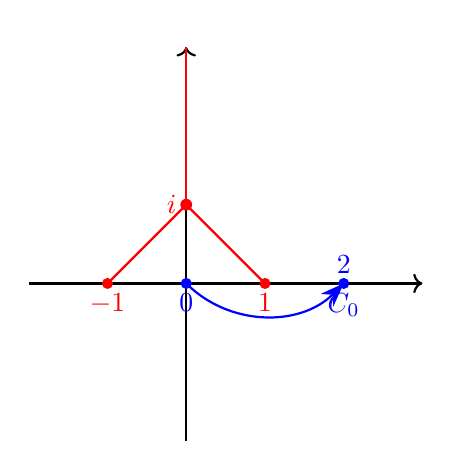
\begin{tikzpicture}
      % Draw the real and imaginary axes
      \draw[thick,->] (-2,0) -- (3,0) node[anchor=north west] {};
      \draw[thick,->] (0,-2) -- (0,3) node[anchor=south east] {};
  
      % Draw the excluded points and lines
      \fill[red] (-1,0) circle (2pt) node[below] {$-1$};
      \fill[red] (1,0) circle (2pt) node[below] {$1$};
      \fill[red] (0,1) circle (2pt) node[left] {$i$};
      \fill[blue] (0,0) circle (2pt) node[below] {$0$};
      \fill[blue] (2,0) circle (2pt) node[above] {$2$};
      \draw[red, thick] (0,1) -- (0,3) node[above, black] {};
      \draw[red, thick] (0,1) -- (1,0) node[above, black] {};
      \draw[red, thick] (0,1) -- (-1,0) node[above, black] {};
      \node at (0,1) [circle,fill,inner sep=1.5pt,red]{};
  
      % Draw the curve from 0 to 2 that goes into the 4th quadrant
      \draw[thick,blue,-{Stealth[length=3mm]}] (0,0) to[out=-45,in=225] (2,0) node[below] {\(C_0\)};
  \end{tikzpicture}
  \caption{2.4.26中\(C_0\)的图示.}
  \label{fig:1}
  \end{figure}

\begin{problem}[2.4.27]
  证明\(\sqrt[4]{(1-z)^3(1+z)}\)能在\(\mathbb{C}\backslash[-1,1]\)上选出单值全纯分支\(f\), 满足\(f(i)=\sqrt2e^{-\frac{\pi}{8}i}\). 求\(f(-i)\).
\end{problem}

\begin{proof}
  任取\(D\)中简单闭曲线\(C\), 只需考虑\(C\)包含\(\pm 1\). 此时\[\Delta_C\mathrm{Arg}f(z)=\frac{3}{4}\Delta_C\mathrm{Arg}(z-1)+\frac14\Delta_C\mathrm{Arg}(1+z)=2\pi.\]
  故\(\sqrt[4]{(1-z)^3(1+z)}\)能在\(D\)上选出单值全纯分支.

  计算
  \begin{align*}
    f(-i)&=f(i)+\Delta_{C_0}\sqrt[4]{(1-z)^3(1+z)}\\
    &=f(i)+f(i)\left(e^{\frac14i\Delta_{C_0}\mathrm{Arg}(1-z)^3(1+z)}-1\right)\\
    &=f(i)+f(i)\left(e^{\frac14i(3\cdot(-\frac{3}{2}\pi)+(-\frac{1}{2}\pi))}-1\right)\\
    &=\sqrt2e^{\frac{5}{8}\pi i},
  \end{align*}
  其中\(C_0\)如图\ref{fig:2}所示.
\end{proof}

\begin{figure}[htbp]
  \centering
  \begin{tikzpicture}
      % Draw the real and imaginary axes
      \draw[thick,->] (-2,0) -- (3,0) node[anchor=north west] {};
      \draw[thick,->] (0,-2) -- (0,3) node[anchor=south east] {};
  
      % Draw the excluded points and lines
      \fill[red] (-1,0) circle (2pt) node[below] {$-1$};
      \fill[red] (1,0) circle (2pt) node[below] {$1$};
      \fill[blue] (0,1) circle (2pt) node[left] {$i$};
      \fill[blue] (0,-1) circle (2pt) node[left] {$-i$};
      \draw[red, thick] (-1,0) -- (1,0) node[above, black] {};
  
      \draw[thick, blue, -{Stealth[length=3mm]}] (0,1) .. controls (2,1) and (2,-1) .. (0,-1) node[pos=0.5, right] {\(C_0\)};
  \end{tikzpicture}
  \caption{2.4.27中\(C_0\)的图示.}
  \label{fig:2}
  \end{figure}

\begin{problem}[2.5.1]
  求将上半平面映为上半平面的分式线性变换, 使得\(\infty\), \(0\), \(1\)分别映为\(0\), \(1\), \(\infty\).
\end{problem}

\begin{solution}
  交比不变:
  \[(w, 0, 1, \infty)=(z,\infty,0,1).\]
  化简得
  \[w=\frac{1}{1-z}.\]

  上半平面是\(\infty\), \(0\), \(1\)和\(0\), \(1\), \(\infty\)的左侧, 因此\(z\mapsto w\)将上半平面映为上半平面.

  故所求变换为\(w=\frac{1}{1-z}\).
\end{solution}

\begin{problem}[2.5.2]
  求将上半平面映为单位圆盘的分式线性变换, 使得\(-1\), \(0\), \(1\)分别映为\(1\), \(i\), \(-1\).
\end{problem}

\begin{solution}
  交比不变:
  \[(w, 1, i, -1)=(z,-1,0,1).\]
  化简得
  \[w=\frac{z-i}{iz-1}.\]

  上半平面是\(-1\), \(0\), \(1\)的左侧, 单位圆盘是\(1\), \(i\), \(-1\)的左侧, 因此\(z\mapsto w\)将上半平面映为单位圆盘.

  故所求变换为\(w=\frac{z-i}{iz-1}\).
\end{solution}

\begin{problem}[2.5.4]
  求将单位圆盘的外部映为右半平面的分式线性变换, 使得
  \begin{enumerate}
    \item \(1\), \(-i\), \(-1\)分别映为\(i\), \(0\), \(-i\);
    \item \(-i\), \(i\), \(1\)分别映为\(i\), \(0\), \(-i\).
  \end{enumerate}
\end{problem}

\begin{solution}
  通过交比不变计算, 再用左右侧说明得到的映射将单位圆盘外部映为右半平面.

  结论:
  \begin{enumerate}
    \item \(w=\frac{z+i}{z-i}\);
    \item \(w=\frac{z-i}{(2-i)z+2i-1}\).
  \end{enumerate}
\end{solution}

\begin{problem}[2.5.5]
  求将上半平面映为自身的分式线性变换, 使得实轴上的\(x_1\), \(x_2\), \(x_3\) \((x_1<x_2<x_3)\)分别映为\(0\), \(1\), \(\infty\).
\end{problem}

\begin{solution}
  交比不变:
  \[(w, 0, 1, \infty)=(z,x_1,x_2,x_3).\]
  化简得
  \[w=\frac{x_2-x_3}{x_2-x_1}\cdot\frac{z-x_1}{z-x_3}.\]

  上半平面是\(x_1\), \(x_2\), \(x_3\)和\(0\), \(1\), \(\infty\)的左侧, 因此\(z\mapsto w\)将上半平面映为上半平面.

  故所求变换为\(w=\frac{x_2-x_3}{x_2-x_1}\cdot\frac{z-x_1}{z-x_3}\).
\end{solution}

\begin{problem}[2.5.13]
  求将\(B(0,1)\)映为自身的分式线性变换, 使得\(\frac12\), \(2\), \(\frac54+\frac34i\)分别映为\(\frac12\), \(2\), \(\infty\).
\end{problem}

\begin{solution}
  通过交比不变, 可求得\[w=\frac{(5-3i)z-4}{4z-(5+3i)}.\]

  为说明这是将\(B(0,1)\)映为自身的变换, 利用\emph{例2.5.16}的表示:
  \[w=\frac{5-3i}{5+3i}\frac{z-\frac{4}{5-3i}}{1-\frac{4}{5+3i}z}.\]

  故所求变换为\(w=\frac{(5-3i)z-4}{4z-(5+3i)}\).
\end{solution}

\begin{problem}[2.5.15]
  求单叶全纯映射, 将除去\([0,1+i]\)的第一象限映为上半平面.
\end{problem}

\begin{solution}
  见图\ref{fig:2.5.15}. \(w=\sqrt{z^4+4}\) (\(\sqrt{\cdot}\)取\(\sqrt{-1}=i\)分支)满足要求.
\end{solution}

\begin{figure}[htbp]
  \centering
  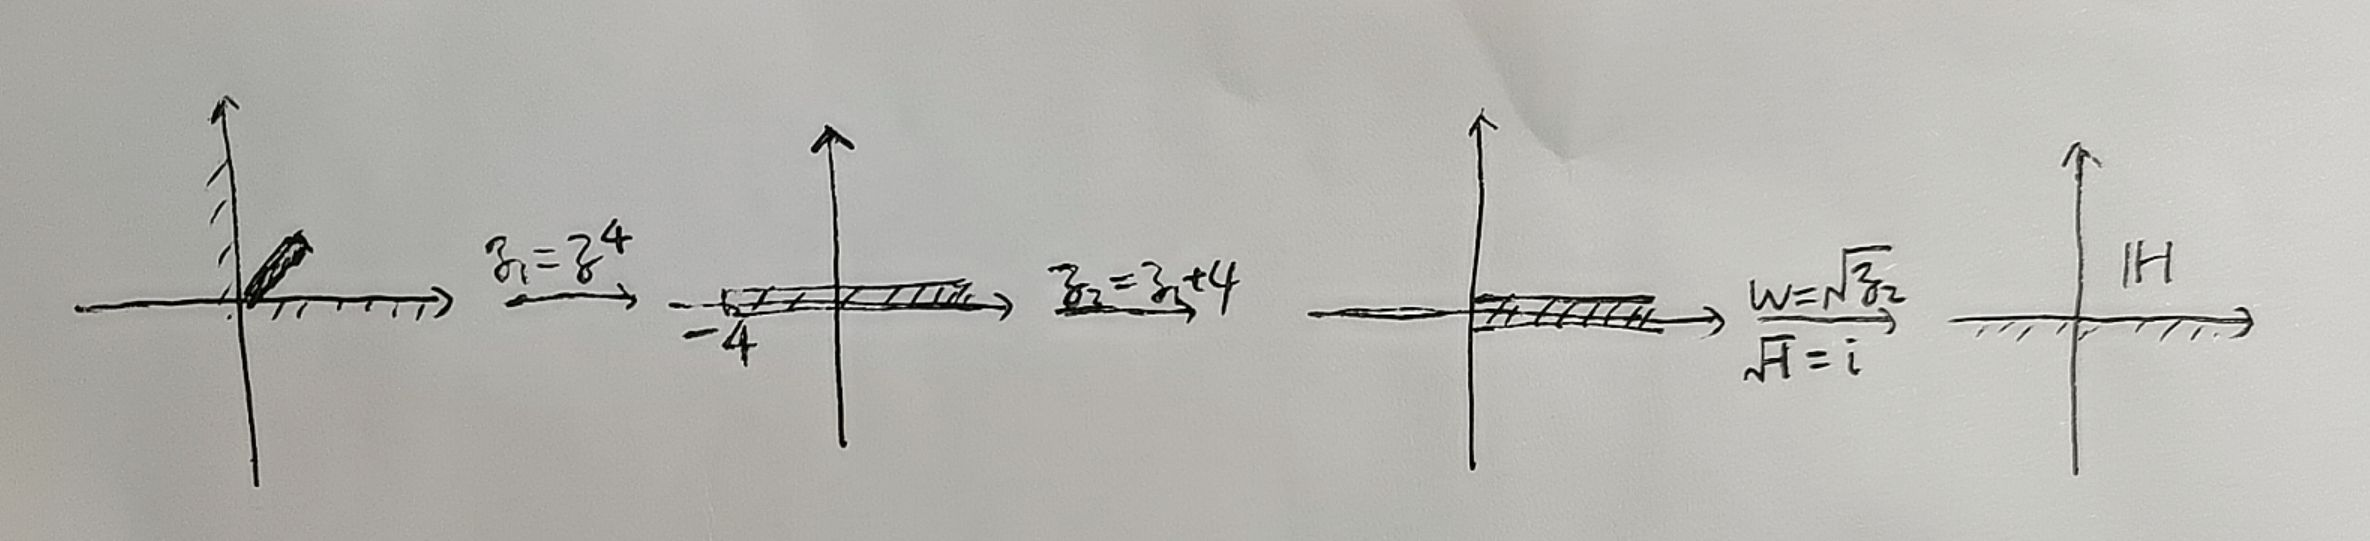
\includegraphics[width=0.8\textwidth]{images/2.5.15.jpg}
  \caption{2.5.15的图示.}
  \label{fig:2.5.15}
\end{figure}

\begin{problem}[2.5.16]
  求单叶全纯映射, 将\(\{z\in\mathbb{C}:-\frac\pi2<\Re z<\frac\pi2,\Im z>0\}\)映为上半平面, 且将\(\frac\pi2\), \(-\frac\pi2\), \(0\)分别映为\(1\), \(-1\), \(0\).
\end{problem}

\begin{solution}
  可以验证\(w=\sin z\)满足要求. 如对三角函数和Joukowsky变换不熟悉, 也可如图\ref{fig:2.5.16}构造.
\end{solution}

\begin{figure}[htbp]
  \centering
  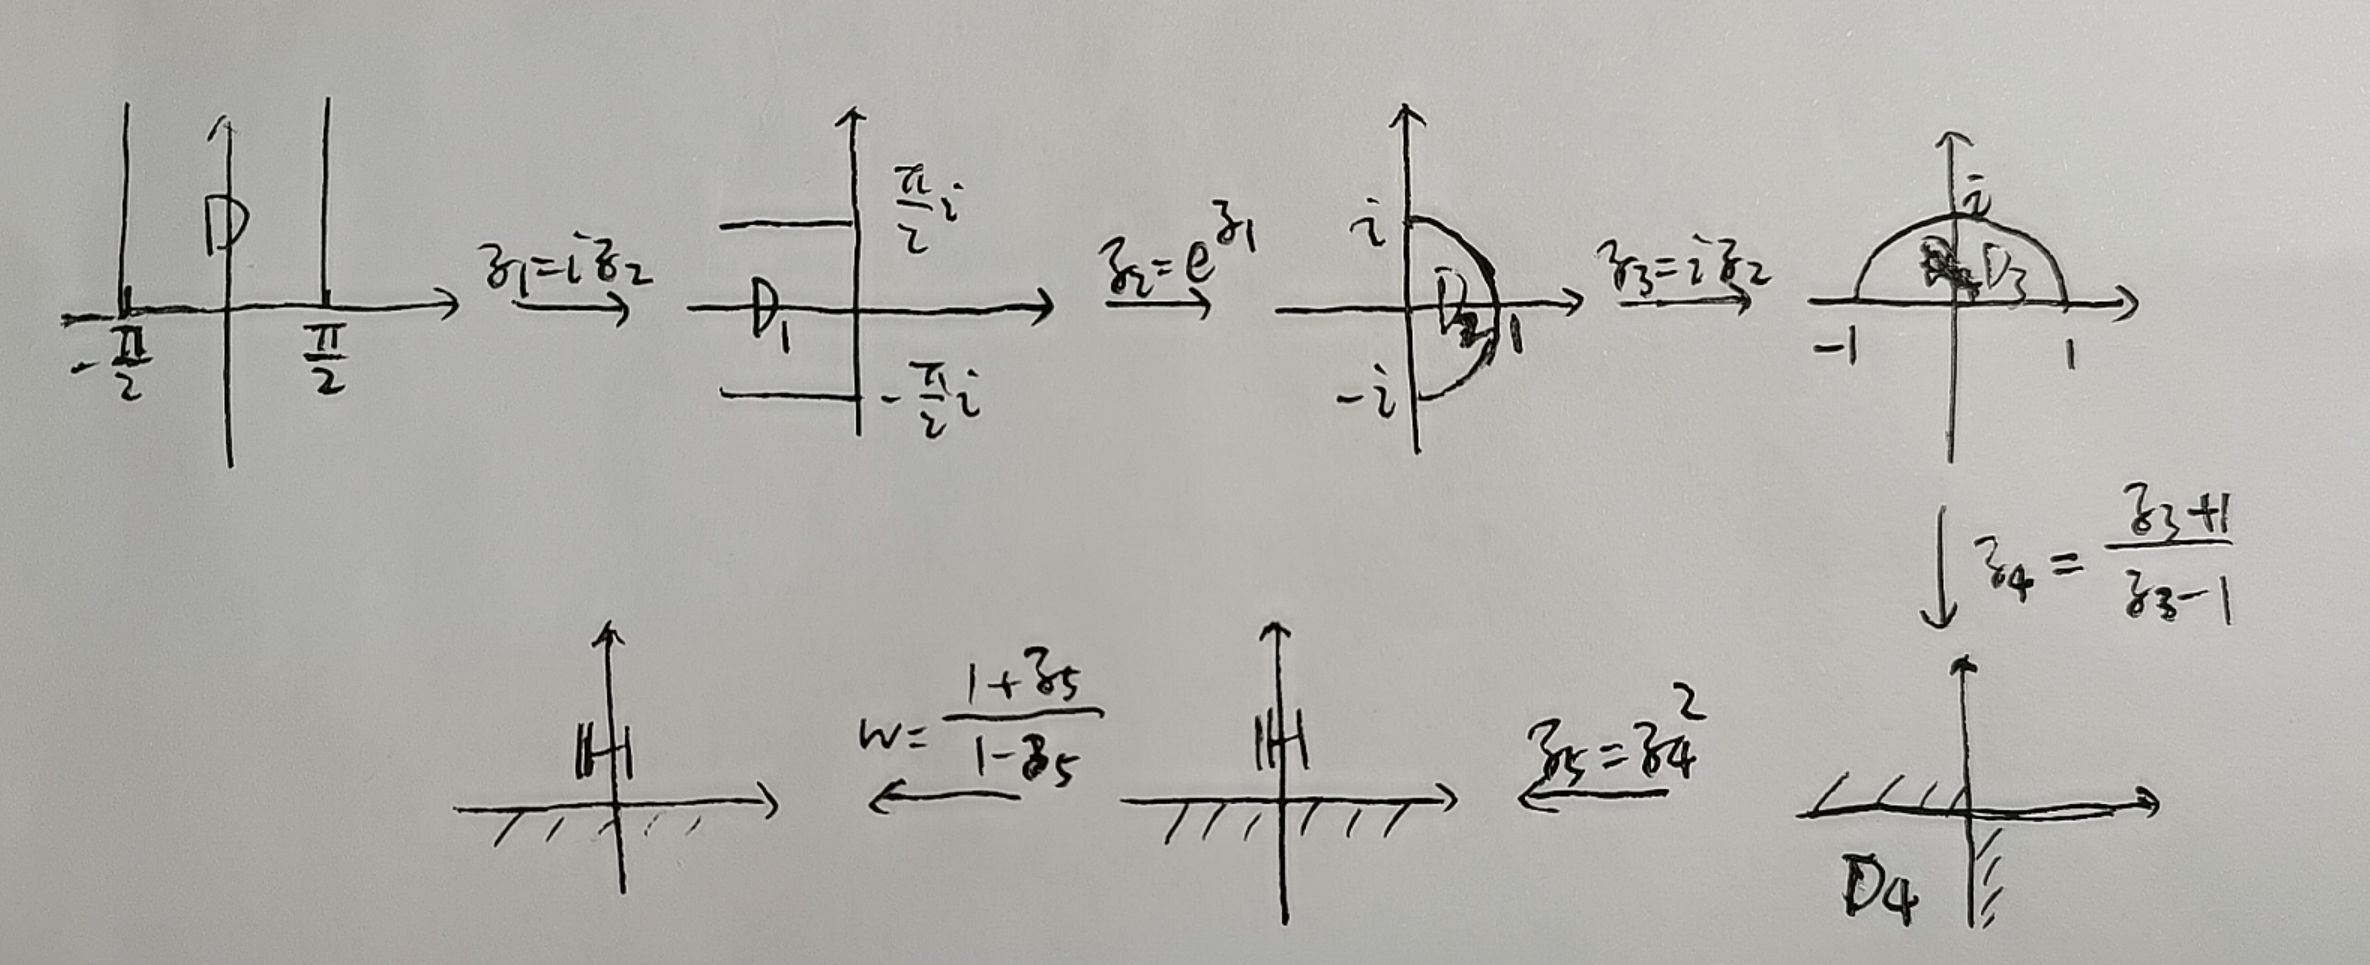
\includegraphics[width=0.8\textwidth]{images/2.5.16.jpg}
  \caption{2.5.16的图示.}
  \label{fig:2.5.16}
\end{figure}

\begin{problem}[2.5.18]
  求单叶全纯映射将\(|z|=1\)与\(|z+\sqrt{3}i|=2\)围成的月牙形域映为单位圆盘.
\end{problem}

\begin{solution}
  见图\ref{fig:2.5.18}. \(w=\frac{3z^2+1}{z^3+3z}\)满足要求.
\end{solution}

\begin{figure}[htbp]
  \centering
  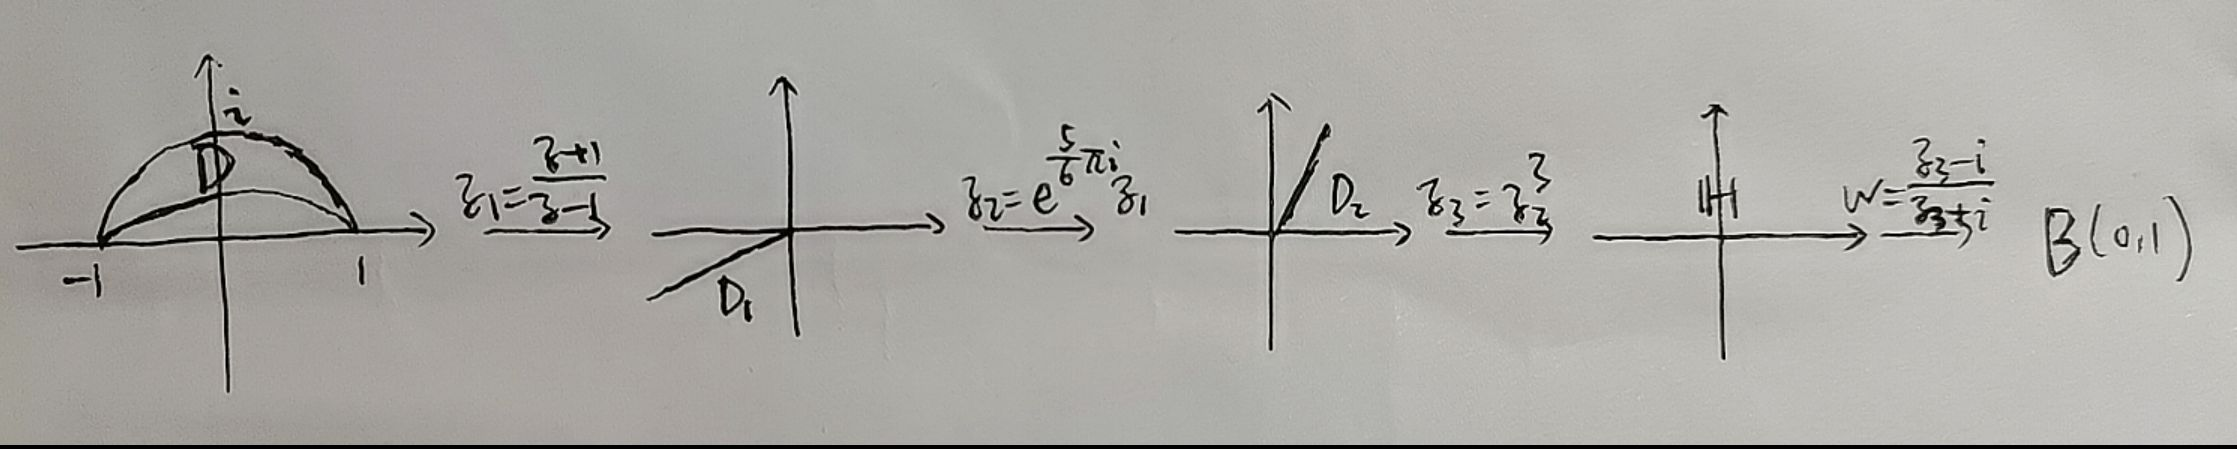
\includegraphics[width=0.8\textwidth]{images/2.5.18.jpg}
  \caption{2.5.18的图示.}
  \label{fig:2.5.18}
\end{figure}

\section{补充题}

\subsection{多值函数计算}

参考第一次习题课习题2.8 (2021年H班期中).

\subsection{共形映射构造}

\begin{problem}[2.5.19]
  求单叶全纯映射将除去\([1,2]\)的单位圆盘外部映为上半平面.
\end{problem}

\begin{solution}
  见图\ref{fig:2.5.19}. \(w=\sqrt{-\frac{(z-1)^2}{(z+1)^2}+\frac19}\) (\(\sqrt{\cdot}\)取\(\sqrt{-1}=i\)分支)满足要求.
\end{solution}

\begin{figure}[htbp]
  \centering
  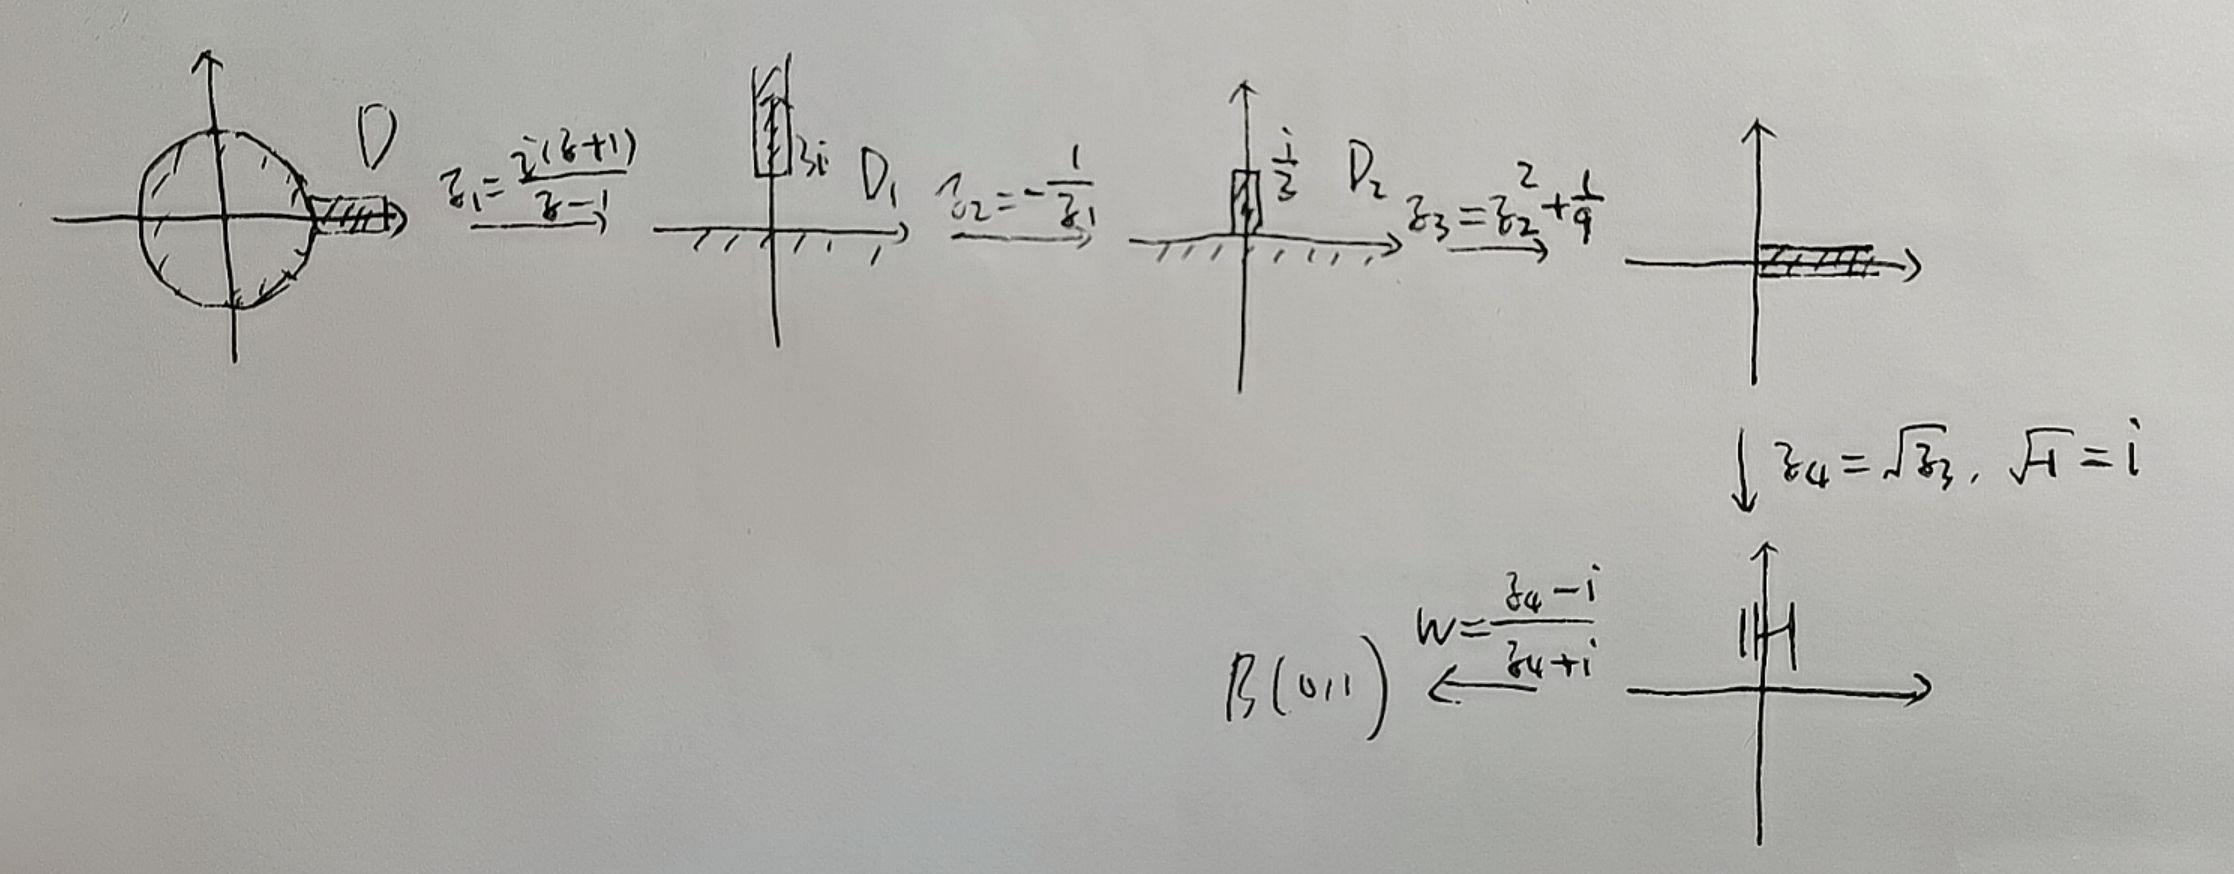
\includegraphics[width=0.8\textwidth]{images/2.5.19.jpg}
  \caption{2.5.19的图示.}
  \label{fig:2.5.19}
\end{figure}

\begin{problem}\label{supp1}
  求共形映射将双曲线\(x^2-y^2=a^2\)的右半支映为单位圆盘, 使得焦点和顶点分别被映为\(0\)和\(-1\).
\end{problem}

\begin{solution}
  见图\ref{fig:supp1}. \(w=1-2a^2z^{-2}\)满足要求.
\end{solution}

\begin{figure}[htbp]
  \centering
  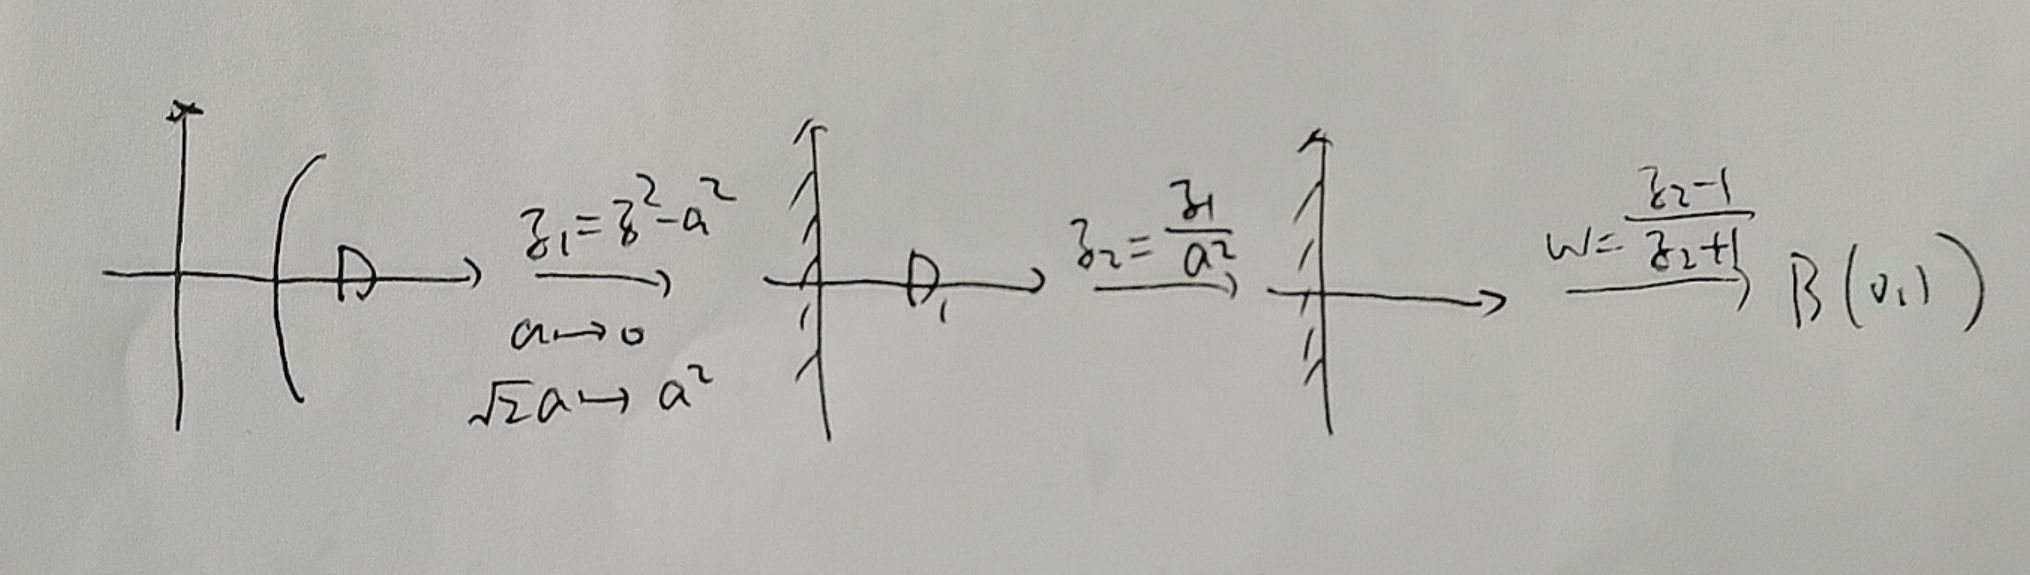
\includegraphics[width=0.8\textwidth]{images/supp1.jpg}
  \caption{题\ref{supp1}的图示.}
  \label{fig:supp1}
\end{figure}

\section{总结}

\subsection{多值函数}

多值函数计算可使用沿曲线增量的方式, 参考课堂内容, 李皓昭老师的讲义, 第一次习题课及本讲义. 关于计算一点处导数的值可参考第一次习题课习题2.8.

\subsection{共形映射构造}

2.5节习题前半部分的题目给出了三个点被映到三个点, 基本做法: 先求出分式线性变换, 再验证其满足其他所有要求. 其中, 求分式线性变换可利用交比不变, 验证满足其他要求可利用分式线性变换的各种性质.

构造共形映射, 可分步作出映射并图示, 最后写出复合映射的表达式, 如用到多值函数, 须注明所取分支. 解题时应注意其他要求. 熟悉一些常见图形的处理办法对解题有帮助.

\end{document}